\documentclass[12pt]{report}
\usepackage[spanish]{babel}
\usepackage[utf8]{inputenc}
\usepackage{amsmath}
\usepackage{amssymb}
\usepackage{amsthm}
\usepackage{graphics}
\usepackage{subfigure}
\usepackage{lipsum}
\usepackage{array}
\usepackage{multicol}
\usepackage{enumerate}
\usepackage[framemethod=TikZ]{mdframed}
\usepackage[a4paper, margin = 1.5cm]{geometry}
\usepackage{graphicx}
\graphicspath{ {images/} }

%En esta parte se hacen redefiniciones de algunos comandos para que resulte agradable el verlos%

\def\proof{\paragraph{Demostración:\\}}
\def\endproof{\hfill$\square$}
\renewcommand{\theenumii}{\roman{enumii}}

%En esta parte se definen los comandos a usar dentro del documento para enlistar%

\newtheoremstyle{largebreak}
  {}% use the default space above
  {}% use the default space below
  {\normalfont}% body font
  {}% indent (0pt)
  {\bfseries}% header font
  {}% punctuation
  {\newline}% break after header
  {}% header spec

\theoremstyle{largebreak}

\newmdtheoremenv[
    leftmargin=0em,
    rightmargin=0em,
    innertopmargin=-2pt,
    innerbottommargin=8pt,
    hidealllines = true,
    roundcorner = 5pt,
    backgroundcolor = gray!60!red!30
]{exa}{Ejemplo}[section]

\newmdtheoremenv[
    leftmargin=0em,
    rightmargin=0em,
    innertopmargin=-2pt,
    innerbottommargin=8pt,
    hidealllines = true,
    roundcorner = 5pt,
    backgroundcolor = gray!50!blue!30
]{obs}{Observación}[section]

\newmdtheoremenv[
    leftmargin=0em,
    rightmargin=0em,
    innertopmargin=-2pt,
    innerbottommargin=8pt,
    rightline = false,
    leftline = false
]{theor}{Teorema}[section]

\newmdtheoremenv[
    leftmargin=0em,
    rightmargin=0em,
    innertopmargin=-2pt,
    innerbottommargin=8pt,
    rightline = false,
    leftline = false
]{propo}{Proposición}[section]

\newmdtheoremenv[
    leftmargin=0em,
    rightmargin=0em,
    innertopmargin=-2pt,
    innerbottommargin=8pt,
    rightline = false,
    leftline = false
]{cor}{Corolario}[section]

\newmdtheoremenv[
    leftmargin=0em,
    rightmargin=0em,
    innertopmargin=-2pt,
    innerbottommargin=8pt,
    rightline = false,
    leftline = false
]{lema}{Lema}[section]

\newmdtheoremenv[
    leftmargin=0em,
    rightmargin=0em,
    innertopmargin=-2pt,
    innerbottommargin=8pt,
    roundcorner=5pt,
    backgroundcolor = gray!30,
    hidealllines = true
]{mydef}{Definición}[section]

\newmdtheoremenv[
    leftmargin=0em,
    rightmargin=0em,
    innertopmargin=-2pt,
    innerbottommargin=8pt,
    roundcorner=5pt
]{excer}{Ejercicio}[section]

%En esta parte se colocan comandos que definen la forma en la que se van a escribir ciertas funciones%

\newcommand\abs[1]{\ensuremath{\lvert#1\rvert}}
\newcommand\divides{\ensuremath{\bigm|}}
\newcommand{\cf}[3]{\ensuremath{#1:#2\rightarrow#3}}

%recuerda usar \clearpage para hacer un salto de página

\begin{document}
    \title{Notas Variedades}
    \author{Cristo Daniel Alvarado}
    \date{\today}
    \maketitle

    \tableofcontents %Con este comando se genera el índice general del libro%

    \setcounter{chapter}{3} %En esta parte lo que se hace es cambiar la enumeración del capítulo%
    
    \chapter{Variedades}
    
    \section{Variedades Topológicas}
    
    Para hacer toda la parte de introducción a varidedades, se hará uso del libro de Loring W. Tu 'An introduction to manifolds'. Hablaremos inicialmente de variedades topológicas. Para entender mejor los conceptos usados a lo largo de la sección, consultar al apéndice A del libro mencionado anteriormente.

    Recordemos varias cosas, Un espacio topológico $M$ es \textbf{segundo numerable} si tiene una base a lo sumo numerable. Una \textbf{vecindad} de un punto $p\in M$ es cualquier conjunto abierto que contenga a $p$. Una \textbf{cubierta abierta de $M$} es una colección $\left\{U_\alpha\right\}_{\alpha\in A}$ de conjuntos abiertos de $M$ tales que $\cup_{\alpha\in A}U_\alpha=M$.

    \begin{mydef}
        Un espacio topológico $M$ es \textbf{localmente euclideano de dimensión n} si todo punto $p\in M$ tiene una vecindad $U\subseteq M$ tal que existe un homeomorfismo $\phi:U\rightarrow V$, donde $V\subseteq\mathbb{R}^n$ es abierto. 
        Al par $(U, \phi:U\rightarrow V)$ se le conoce como una \textbf{carta}, $U$ es una \textbf{vecindad coordenada} o \textbf{conjunto abierto coordenado}, y $\phi$ es el mapeo \textbf{mapeo coordenado} o \textbf{sistema coordenado sobre $U$}.

        Decimos que una carta $(U,\phi)$ \textbf{está centrada en $p\in U$} si para $\phi(p)=0$. Una carta $(U,\phi)$ \textbf{alrededor de $p$} simplemente significa que $(U,\phi)$ es una carta y que $p\in U$.
    \end{mydef} 

    \begin{mydef}
        Una \textbf{Variedad Topológica de dimensión n} es un espacio topológico localmente euclideano de dimensión n, Hausdorff y segundo numerable.
    \end{mydef}

    Recordamos que la condición de Hausdorff y la segunda numerabilidad son propiedades hereditarias, esto es, son heredadas a los subespacios de estos espacios topológicos. Un subespacio de un espacio Hausdorff es Hausforff y un subespacio de un espacio segundo numerable es segundo numerable. Así que de forma inmediata, como $\mathbb{R}^n$ es Hausdorff y segundo numerable, cualquier subespacio de él es automáticamente Hausdorff y segundo numerable.

    \begin{exa}
        El espacio euclideano $\mathbb{R}^n$ es una variedad topológica de dimensión n, pues pues es un espacio topológico localmente euclideano, pues para todo $p\in\mathbb{R}^n$ existe $\phi=\textup{id}_{\mathbb{R}^n}$ homeomorfismo de $\mathbb{R}^n$ en $\mathbb{R}^n$, además $\mathbb{R}^n$ es Hausdorff y segundo numerable.
    \end{exa}

    \begin{exa}
        Considere la gráfica de la función $f\mathbb{R}\rightarrow\mathbb{R}$, $x\mapsto x^{2/3}$. Su gráfica tiene la siguiente forma:
        %insertar gráfica%
        Su gráfica (denotada por $\Gamma(f)$) es una variedad topológica, esto en virtud de ser un subespacio de $\mathbb{R}^2$, el cual es Hausdorff y segundo numerable. Y es localmente euclideano ya que es homeomorfo a $\mathbb{R}$, usando el mapeo $\pi:\mathbb{R}^2\rightarrow\mathbb{R}$, $(x,x^{2/3})\mapsto x$.
    \end{exa}

    \begin{exa}
        Considere la cruz como subconjunto de $\mathbb{R}^2$. Claramente es Hausdorff y segundo numerable. Probaremos que no es una variedad topológica de dimensión 1 ó 2. Suponga que lo es, entonces para $p\in M$ (la intersección de la cruz) existe un mapeo $\phi:U\rightarrow V$, donde $U\subseteq M$ ($M$ es el espacio topológico) con $V\subseteq \mathbb{R}^n$, donde $n\in\mathbb{N}$. Podemos suponer que $U$ es abierto conexo (si no es conexo, basta tomar una bola tal que esté contenida en $U$). Notemos que $U/\left\{p\right\}$ es un conjunto que tiene 4 componentes conexas. Si
        \begin{itemize}
            \item $n=1$, como los abiertos conexos en $\mathbb{R}$ son intervalos conexos, al quitarles un punto del interior, se tiene que $V/\left\{\phi(p)\right\}$ tiene dos componentes conexas.
            \item $n>1$, como a los conexos abiertos de $\mathbb{R}^n$ con $n>1$ al quitarles un punto siguen siendo conexos, se tiene que $V/\left\{\phi(p)\right\}$ tiene una componente conexa.
        \end{itemize}
        como los homeomorfismos mandan componentes conexas en componentes conexas, no puede suceder que la imagen de $U/\left\{p\right\}$ el cual es $V/\left\{\phi(p)\right\}$ tenga 2 o una componente conexa. Luego el espacio topológico $M$ no es localmente euclideano y por tanto, no es variedad topológica.
    \end{exa}

    \section{Compatibilidad de Cartas}

    Sea $M$ una variedad topológica y considere $(U, \phi:U\rightarrow \mathbb{R}^n)$ y $(V, \psi:V\rightarrow \mathbb{R}^n)$ dos cartas de la variedad topológica $M$.

    \begin{mydef}
        Dadas dos cartas de una variedad topológica (usando la notación de lo escrito anteriormente), decimos que son \textbf{$C^{\infty}$-compatibles} si los dos mapeos
        \begin{equation}
            \begin{split}
                \phi\circ\psi^{-1}:&\psi(U\cap V)\rightarrow \phi(U\cap V)\\
                \psi\circ\phi^{-1}:&\phi(U\cap V)\rightarrow \psi(U\cap V)\\
            \end{split} 
        \end{equation}
        son $C^{\infty}$. Estos dos mapeos son llamados \textbf{funciones de transición} entre las cartas.
    \end{mydef}

    \begin{obs}
        En el contexto de la definición anterior, en caso de que la intersección de las dos cartas sea vacía, las cartas serán en automático $C^{\infty}$-compatibles.

        Para simplificar la notación, escribiremos
        \begin{equation*}
            U_{\alpha\beta}=U_{\alpha}\cap U_{\beta}
        \end{equation*}
        y
        \begin{equation*}
            U_{\alpha\beta,\gamma}=U_{\alpha}\cap U_{\beta}\cap U_{\gamma}
        \end{equation*}
    \end{obs}

    Como nuestro interés va solo sobre cartas $C^{\infty}$-compatibles, seguidamente vamos a omitir la mención de $C^{\infty}$ y hablaremos simplemente de cartas compatibles.

    \begin{mydef}
        Un \textbf{Atlas $C^{\infty}$} o simplemente un \textbf{atlas} en un espacio localmente euclideano, es una colección $\mathbb{U}=\left\{(U_\alpha, \phi_\alpha)\right\}$ de cartas $C^{\infty}$-compatibles a pares que cubren a $M$, es decir tales que $M=\cup_{\alpha}U\alpha$. 
    \end{mydef}

    \begin{obs}
        La $C^{\infty}$-compatibilidad de cartas es una relación reflexiva, simétrica, pero no es transitiva. En efecto.
    \end{obs}
    \begin{proof}
        Sea $M$ un espacio localmente euclideano. 
    \end{proof}

    \begin{obs}
        Si $M$ y $N$ son variedades suaves, entonces $M\times N$ con su topología producto es una variedad suave.
    \end{obs}

    \begin{propo}
        Si $\left\{(U_{\alpha},\phi_{\alpha})\right\}$ y $\left\{(V_\beta,\psi_\beta)\right\}$ son atlas para $M$ y $N$, respectivamente, entonces
        \begin{equation*}
            \left\{(U_\alpha\times V_\beta,\phi_\alpha\times\psi_\beta:U_\alpha\times V_\beta\rightarrow M\times N)\right\}
        \end{equation*}
        es un atlas para $M\times N$.
    \end{propo}

    \begin{exa}
        $T^2=S^1\times S^1$. Y el $n$-toro $T^n=\underbrace{S^1\times S^1}_{\textup{n-veces}}$ son ejemplos de variedades suaves.
    \end{exa}

    \setcounter{chapter}{5}

    \chapter{Funciones suaves sobre una variedades}

    \section{Introducción}

    \begin{mydef}
        Sea $M$ una variedad de dimensión $n$. Una función $f:M\rightarrow \mathbb{R}$ se dice que \textbf{es una función $C^\infty$ en $p\in M$} si existe una carta $(U,\phi)$ que contenga a $p$ tal que $f\circ \phi^{-1}$ es $C^\infty$ en $\phi(p)$. La función $f$ se dice que es \textbf{$C^\infty$ en $M$} si es $C^\infty$ en cada punto de $M$.
    \end{mydef}

    \begin{figure}
        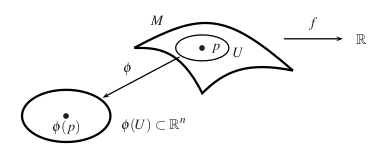
\includegraphics[scale = 0.75]{f_suaves.png}
        \centering
        \caption{Función $C^\infty$.}
    \end{figure}

    Notemos que la definición de suavidad de una función $f$ en u punto es independiente de de la carta $(U,\phi)$, pues si $f\circ \phi^{-1}$ es $C^\infty$ en $\phi(p)$ y $(V,\psi)$ es otra carta sobre $p\in M$, entonces en $\psi(U\cap V)$:

    \begin{equation*}
        f\circ \psi^{-1}=(f\circ\phi^{-1})\circ(\phi\circ\psi^{-1})
    \end{equation*}

    las cual es $C^\infty$ en $\psi(p)$.

    Se denota al conjunto de \textbf{la funciones suaves sobre una variedad suave $M$} por:

    \begin{equation*}
        C^\infty(M)=\left\{\textup{conjunto de todas las funciones $C^\infty$ sobre $M$}\right\}
    \end{equation*}

    Sean $M^m$ y $N^n$ variedades suaves, $h\in C^\infty(M)$ y $F:N\rightarrow M$ funciones. Se define el \textbf{pullback de $h$ bajo $F$} como la función

    \begin{equation*}
        F^*h=h\circ F
    \end{equation*}

    \begin{mydef}
        Sean $M$ y $N$ variedades suaves  de dimensión $n$ y $m$, respectivamente. Una función continua $f:N\rightarrow M$ es \textbf{$C^\infty$ en un punto $p\in N$} si existen cartas $(V,\psi)$ alrededor de $F(p)$ en $M$ y $(U,\phi)$ alrededor de $p$ en $N$ tales que la composición
        \begin{equation*}
            \psi \circ F\circ \phi^{-1}
        \end{equation*}
        el cual es un mapeo del abierto $\phi(F^{-1}(V)\cap U)$ subcojunto de $\mathbb{R}^n$ y va a $\mathbb{R}^m$, es $C^\infty$ en $\phi(p)$.

        Se die que $F$ \textbf{es $C^\infty$} si es $C^\infty$ en todo punto de $N$. Este es un \textbf{difeomorfismo} si este es biyectivo y tanto $F$ como $F^{-1}$ son $C^\infty$.
    \end{mydef}

    \begin{figure}
        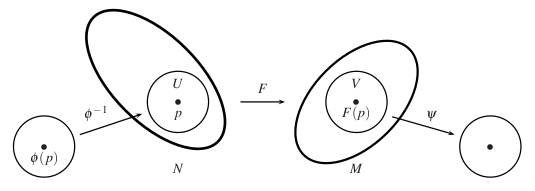
\includegraphics[scale = 0.75]{Pullback.png}
        \centering
        \caption{Función $F:N\rightarrow M$ entre dos variedades.}
    \end{figure}

    \begin{exa}
        Si $(U,F)$ es una carta en el atlas de $M$, entonces $F$ y $F^{-1}$ son $C^\infty$.
    \end{exa}

    \begin{proof}
        En efecto, notemos que $U\subseteq\mathbb{R}^n$ abierto es variedad de dimensión $n$. En particular, podemos interpretar a $F$ como el mapeo entre las variedades $U$ y $F(U)$. de forma inmediata se sigue que $F$ es difeomorfismo.
    \end{proof}

    %Esta es la proposicicón 6.11
    \begin{propo}
        Sea $U\subseteq M$ abierto. Si $F:U\rightarrow F(U)\subseteq\mathbb{R}^n$ es un difeomorfismo sobre su imagen, entonces $(U,F)$ es una carta en el atlas de $M$.
    \end{propo}

    \setcounter{chapter}{7}
    \chapter{El Espacio Tangente}

    \section{Vectores Tangentes}

    %Checar página 87 (o 106) del Introduction to differential forms

    \begin{mydef}[\textbf{Coordenadas estándar de $\mathbb{R}^n$}]
        Para cada cada $i=1,\dots,n$, se definen las funciones \textbf{coordenadas estándar de $\mathbb{R}^n$} como
        \begin{equation*}
            p=(p_1,\dots, p_n)\mapsto r_i(p)=p_i
        \end{equation*}
    \end{mydef}

    Esto se usará para evitar conflictos más adelante con la notación de coordenadas locales sobre una variedad.

    \begin{mydef}[\textbf{Derivada direccional}]
        Sea $M$ una variedad y $p\in M$. Consideremos $\alpha:I\rightarrow M$ función continua (dónde $I$ es un intervalo conexo tal que $0\in I$) y $f:M\rightarrow \mathbb{R}$ función diferenciable sobre la variedad. Entonces $f\circ \alpha$ es una función de $I$ en $\mathbb{R}$. Se denota por
        \begin{equation*}
            \alpha'(0)[f]=\frac{d}{dt}(f\circ\alpha)(t)\Big|_{t=0}
        \end{equation*}
        llamada \textbf{derivada direccional de $f$ en la dirección de $\alpha'(0)$}.
    \end{mydef}

    Para dar la definición de vector tangente, tenemos que retomar el concepto de de \textbf{germen} de una función $C^\infty$. Lo hacemos tomando una función $\cf{f}{M}{\mathbb{R}}$ y un punto $p\in M$. Decimos que $\cf{g}{M}{\mathbb{R}}$ es equivalente a $f$, si coinciden en una vecindad de $p$.

    El conjunto de gérmenes de funciones reales $C^\infty$ en un punto $p\in M$ es denotado por $C_p^\infty(M)$. Esta es un algebra sobre $\mathbb{R}$.

    Generalizando la derivación en un punto en $\mathbb{R}^n$, definimos la \textbf{derivación en un punto en una variedad $M$}, o \textbf{derivación puntual de $C_p^\infty(M)$} que sea un mapeo lineal $\cf{D}{C_p^\infty(M)}{\mathbb{R}}$ tal que
    \begin{equation*}
        D(fg)=(Df)g(p)+f(p)Dg
    \end{equation*}

    \begin{mydef}
        Sea $M$ una variedad suave. Un \textbf{vector tangente en un punto $p\in M$} es una derivación en $p$.
    \end{mydef}

    Retomando la parte de la derivada direccional, tomemos una carta $(\phi, U)$ tal que $p\in U$. Tenemos entonces que

    \begin{equation}
        \begin{split}
            \alpha'(0)[f]&=\frac{d}{dt}(f\circ\alpha)(t)\Big|_{t=0}\\
            &=\frac{d}{dt}(f\circ\phi^{-1}\circ\phi\circ\alpha)(t)\Big|_{t=0}\\
            &=\frac{d}{dt}((f\circ\phi^{-1})\circ(\phi\circ\alpha))(t)\Big|_{t=0}\\
            &=\sum_{i=1}^{n}\frac{d}{dr^i}(f\circ\phi^{-1})\Big|_{\phi(p)}\cdot \frac{dr^i}{dt}\Big|_{t=0}
        \end{split}
    \end{equation}
    pues, en este caso vemos que $\cf{\phi\circ\alpha}{I}{\mathbb{R}^n}$, tal que $t\mapsto (r^1(t),\dots,r^n(t))$ ($r^i$ son las funciones coordenadas de $\mathbb{R}^n$), para todo $t\in I$, donde $\cf{\phi}{U}{\mathbb{R}^n}$.
    
    De esta forma, se tiene que
    \begin{equation*}
        \begin{split}
            \alpha'(0)[f]&=\sum_{i=1}^{n}\frac{d}{dr^i}(f\circ\phi^{-1})\Big|_{\phi(p)}\cdot \frac{dr^i}{dt}\Big|_{t=0}
        \end{split}
    \end{equation*}

    definimos las coordenadas locales de la variedad $M$ en la carta $(\phi, U)$, como:

    \begin{equation*}
        x^i:=\cf{r^i\circ\phi}{U}{\mathbb{R}}
    \end{equation*}

    de esta forma, se sigue que

    \begin{equation*}
        \frac{\partial}{\partial x^i}\Big|_{p}f=\frac{\partial}{\partial r^i}\Big|_{\phi}f\circ\phi^{-1}\in\mathbb{R}
    \end{equation*}

    de esta forma, (6.1) es escribe como:

    \begin{equation*}
        \alpha'(0)[f]=\sum_{i=1}^{n}\frac{\partial}{\partial x^i}\Big|_{p}f\cdot\frac{dr^i}{dt}\Big|_{t=0}
    \end{equation*}

    (de alguna forma, lo que se hace es definir la derivación de una función en dirección de una curva sobre la variedad). Podemos ver entonces a $\frac{\partial}{\partial x^i}\Big|_{p}$ como un operador lineal que va de $C_p^{\infty}(M)$ en $\mathbb{R}$. es decir, es una derivación.

    \begin{obs}
        Airmamos que $d\phi^{-1}_{\phi(p)}(\frac{\partial}{\partial r^i}\Big|_{\phi(p)})=\frac{\partial}{\partial x^i}\Big|_{p}$.
    \end{obs}

    \begin{proof}
        No se probará, pues no se entendió en lo absoluto lo que hizo el profesor.
    \end{proof}

    De ahora en adelante, no habrá defininciones formales, simplemente se intenta dar una idea breve de lo que sucede para llegar a formas diferenciales sobre variedades.

    \begin{obs}
        Con estas ideas, afirmamos que
        \begin{equation*}
            \frac{\partial}{\partial x^i}\Big|_{p}x^j=\delta_{ij}
        \end{equation*}
    \end{obs}

    \begin{proof}
        En efecto, observemos que
        \begin{equation*}
            \begin{split}
                \frac{\partial}{\partial x^i}x^j&=\frac{\partial}{\partial r^i}\Big|_{\phi(p)}(x^j\circ\phi^{-1})\\
                &=\frac{\partial}{\partial r^i}\Big|_{\phi(p)}(r^j\circ\phi\circ\phi^{-1})\\
                &=\frac{\partial}{\partial r^i}\Big|_{\phi(p)}(r^j)\\
                &=\frac{\partial r^j}{\partial r^i}\Big|_{\phi(p)}\\
                &=\delta_{ij}\\
            \end{split}
        \end{equation*}
    \end{proof}

    \section{El diferencial de un mapeo}

    \begin{mydef}
        Sea $\cf{F}{N}{M}$ un mapeo $C^\infty$ entre dos variedades suaves. Para cada punto $p\in N$, el mapeo $F$ induce un mapeo lineal entre espacios tangentes, llamado \textbf{su diferencial en $p$}, dado como
        \begin{equation*}
            F_*:T_pN\rightarrow T_{F(p)}M
        \end{equation*}
        como sigue. Si $X_p\in T_pN$, entonces $F_*(X_p)$ es el vector tangente en $T_{F(p)}M$ definido por
        \begin{equation}
            (F_*(X_p))[f]:=X_p[f\circ F]\in\mathbb{R},\quad\textup{para }f\in C_{F(p)}^\infty(M)
        \end{equation}
        Aquí, $f$ es un gérmen en $F(p)$, representado por una función $C^\infty$ en una vecindad de $F(p)$. En la ecuación (8.2), la definición es independiente del gérmen y el representante de la función (cosa que se tiene que probar en el siguiente ejercicio)
    \end{mydef}

    \begin{excer}
        Pruebe que $F_*(X_p)$ es una derivación en $F(p)$ y que el mapeo $F_*:T_pN\rightarrow T_{F(p)}M$ es lineal.
    \end{excer}

    \setcounter{propo}{8}

    \begin{propo}
        Sea $(U,\phi)=(U,x^1,\cdots,x^n)$ una carta alrededor de un punto $p\in M$, siendo $M$ una variedad. Entonces
        \begin{equation*}
            \phi_*\left(\frac{\partial}{\partial x^i}\Big|_{p}\right)=\frac{\partial}{\partial r^i}\Big|_{\phi(p)}
        \end{equation*}
    \end{propo}

    \begin{proof}
        Sea $f\in C_{\phi(p)}^\infty$, entonces
        \begin{equation*}
            \begin{split}
                \phi_*\left(\frac{\partial}{\partial x^i}\Big|_{p}\right)f\\
                &=\frac{\partial}{\partial x^i}\Big|_{p}(f\circ\phi)\\
                &=\frac{\partial}{\partial r^i}\Big|_{\phi(p)}(f\circ\phi\circ\phi^{-1})\\
                &=\frac{\partial}{\partial r^i}\Big|_{\phi(p)}f\\
            \end{split}
        \end{equation*}
    \end{proof}

    \begin{propo}
        Si $(U,\phi)$ es una carta que contiene a $p\in M$, entonces el espacio tangente $T_pM$ tiene como base
        \begin{equation*}
            \frac{\partial}{\partial x^1}\Big|_p,\dots,\frac{\partial}{\partial x^n}\Big|_p
        \end{equation*}
    \end{propo}

    \begin{propo}[\textbf{Matriz de transición para vectores coordenados}]
        Dadas cartas $(U,\phi)=(U,x^1,\dots,x^n)$ y $(V,\psi)=(V,y^1,\dots,y^n)$ sobre una variedad $M$ tales que $U\cap V\neq \emptyset$, entonces
        \begin{equation*}
            \frac{\partial}{\partial x^j}=\sum_{i=1}^n\frac{\partial y^i}{\partial x^j}\frac{\partial}{\partial y^i},\quad \forall j\in\left\{1,\dots,n\right\}
        \end{equation*}
        en $U\cap V$.
    \end{propo}

    \newpage

\end{document}